\chapter{Leitfaden Experteninterviews}
\label{chap:expert-interviews-leitfaden}

Dieser Leitfaden beschreibt den Plan, nach dem in den Experteninterviews vorgegangen wird.

\section{Übersicht}

Eine Übersicht über den Rahmen der Experteninterviews ist in \cref{tab:expert-interviews-übersicht} gegeben sowie ein Zeitplan in \cref{tab:expert-interviews-zeitplan}.

\begin{table}[!ht]
  \centering
  \begin{tabular}{|l | p{9cm}|}
    \hline
    Ziel & Bewertung der Nützlichkeit des MMF/ARH bei Migration zu Microservices im Spezialfall jadice flow \\ \hline
    Art des Interviews & Semi-Strukturiert, Einzelinterviews \\ \hline
    Interviewte & Product Owner, Softwarearchitekt, Softwareentwickler \\ \hline
    Interviewer & Axel Herrmann \\ \hline
    Dauer &ca. 45 min \\ \hline
    Datum & 26.02.2024 \& 29.02.2024 \\ \hline
    Ort & Büro levigo/ Online-Meeting TODO \\ \hline
  \end{tabular}
  \caption[Übersicht Experteninterviews]{
    Übersicht über die Experteninterviews
  }
  \label{tab:expert-interviews-übersicht}
\end{table}

\begin{table}[!ht]
	\centering
	\begin{tabular}{m{4.1cm} m{8cm} c}
		\toprule
		\textbf{Schritt} & \textbf{Ziel} & \textbf{Dauer} \\ \midrule
		Einleitung & Begrüßung, Zustimmung zur Verarbeitung und Auf\-zeich\-nung, Erfassung grundlegender Daten & 5 min \\
		Gewünschte Qualitäten ei\-nes \gls{mmf} allgemein & Einschätzung ohne Bezug auf MMF/ARH & 10 min \\
		Verständnisfragen zu MMF/\-ARH & Verständnisprobleme eliminieren, damit spätere Fra\-gen auf vergleichbarem Wissensstand durchgeführt werden können & 10 min \\
		Evaluation MMF/ARH & Hauptteil. Bewertung der in dieser Arbeit durch\-ge\-führ\-ten Anwendung des ARH auf \jf & 20 min \\
		\bottomrule
	\end{tabular}
	\caption[Zeitplan Experteninterviews]{
		Zeitplan der Experteninterviews
	}
	\label{tab:expert-interviews-zeitplan}
\end{table}


\section{Einleitung}

Zu Beginn oder je nach Betrachtung vor Beginn der Experteninterviews werden einige Formalitäten geklärt.
Dabei wird nach einem klaren, strukturiertem Plan vorgegangen:

\begin{enumerate}
	\item Zustimmung zur Aufzeichnung des Interviews und zur Verarbeitung der Daten
	\item Übersicht über die Präambel
	\item Start der Aufzeichnung
	\item Dem Interviewten seine Rolle nennen (da einzelne Interviewte teilweise mehrere Rollen innehaben)
	\item Professionelle Erfahrung in der Informatik in Jahren
	\item Erfahrung mit Microservices in Jahren
	\item Arbeit an dem Produkt (\emph{jadice server} zählt als Vorgänger ebenfalls zu \jf) in Jahren
\end{enumerate}

\section{Evaluation}

Nach der Einleitung kann der Hauptteil der Experteninterviews beginnen.
Im Gegensatz zu den Aussagen und Fragen in der Einleitung ist bei den folgenden Fragen der Wortlaut wichtig, da die Fragen teilweise offen sind.
Deswegen werden die Fragen so wie hier beschrieben gestellt.

\subsection{Gewünschte Qualitäten eines MMF allgemein}

Versetzen Sie sich zurück in die Zeit, in der die Planung der Migration von \emph{jadice server} zu einer \acrlong{msa} bevorstand, aus der dann \jf entstanden ist.
Sie suchen nach einem Werkzeug, einer Software in einer beliebigen Form, das Sie bei der Migration zu Microservices unterstützen soll.

\begin{enumerate}
	\item Welche Aufgaben soll ein solches Werkzeug für Sie übernehmen bzw. bei welchen soll es Sie unterstützen?
	\item Falls noch nicht in der letzten Frage erläutert: Welche Qualitäten soll das Werkzeug mich sich bringen?
\end{enumerate}

\subsection{Verständnisfragen zu MMF/ARH}

\begin{enumerate}
	\item Hatten Sie Probleme, Teile des Informationsmaterials zu verstehen, soll ich bestimmte Details genauer erläutern?
	\item Falls Probleme bestehen: Was sollte am Informationsmaterial verbessert werden?
	\item Falls nicht durch Besprechung der Probleme bereits geschehen: Kurze Zusammenfassung über die zwei enthaltenen Migrationsverfahren.
\end{enumerate}

\subsection{Evaluation MMF/ARH}

\begin{enumerate}
	\item Wie schätzen Sie die Nützlichkeit der vorgestellten Methoden im Bezug auf das Refactoring von \jf mit diesen mit Ziel der Verbesserung der Granularität, des Kommunikationsmodells und des Netzwerk-Overheads ein?
	\item Wie passend schätzen Sie die folgenden Best Practices und Patterns für \jf ein?
	\item Würden Sie nach den Ihnen verfügbaren Informationen die Verwendung des MMF/ARH für \jf zum jetzigen Zeitpunkt als sinnvoll und potentiell gewinnbringend betrachten?
	\item Hätten Sie nach den Ihnen verfügbaren Informationen die Verwendung des MMF/ARH für die Migration von \emph{jadice server} zu Microservices in der Vergangenheit  als sinnvoll und potentiell gewinnbringend betrachten?
\end{enumerate}





\chapter{Präambel Experteninterviews}
\label{chap:expert-interviews-preamble}

In diesem Dokument werden die allgemeinen Richtlinien und ethischen Erwägungen für die Experteninterviews dieser Fallstudie beschrieben.

\section{Ziel der Studie}

Wir erforschen das toolunterstützte Refactoring von Microservices mit dem Tool \emph{\acrlong{arh}} nach dem \emph{\acrlong{mmf}}.
Ziel dieser Fallstudie ist es, diese am Produkt \jf der Firma \emph{levigo solutions} zu testen und diesen Test zu evaluieren.
Damit soll auf der einen Seite eine potentielle Überarbeitung von \jf angestoßen werden und auf der anderen Seite Erkenntnisse über die Effektivität des Frameworks und Tools gewonnen werden, die in Zukunft bei der Weiterentwicklung dieser helfen sollen.

Das Framework hat allgemein das Ziel, die Lücke zwischen Industrie und Akademie zu verringern, indem wissenschaftliche Methoden für die Migration zu Microservices-Architekturen in einem webbasierten Tool kategorisiert und so für die Industrie zugänglich gemacht werden.

\section{Ziel der Experteninterviews}

In diesen Interviews soll Evaluation der Anwendung des Frameworks und Tools auf \jf in dieser Arbeit stattfinden.
Dabei soll sowohl eine allgemeine Bewertung des Konzepts des Frameworks durchgeführt werden als auch die spezielle Anwendung des Tools mit \jf, die in dieser Arbeit stattgefunden hat.

\section{Vertraulichkeit und Anonymität}
Alles, was in den Interviews gesagt wird, wird streng vertraulich behandelt und ohne die Erlaubnis der Teilnehmer an niemanden außerhalb unseres Forschungsteams weitergegeben.
Die Ergebnisse werden vor der Veröffentlichung aggregiert und anonymisiert.
Einzelne Aussagen können in keinster Weise auf einen Mitarbeiter zurückgeführt werden.
Auch nach dem Interview haben die Teilnehmer die Möglichkeit, Aussagen vor der Auswertung auszuschließen oder zu schwärzen.
Die vollständigen Interviewtranskripte werden NICHT veröffentlicht.

\section{Interviewprozess und Analyse}
Die Befragten werden über das allgemeine Thema der Studie informiert, so dass sie damit vertraut sind und sich vorab informieren können, falls sie dies wünschen.
Die Dauer des Interviews wird auf 45 Minuten geschätzt.
Ich bitte Sie um Ihre Erlaubnis, das Interview für die Transkription aufzuzeichnen.
Die schriftliche Abschrift wird dem Teilnehmer zur endgültigen Genehmigung zurückgeschickt.
Dies ist die letzte Möglichkeit, Aussagen aus dem Interview zu entfernen oder zu kürzen.
Danach wird die Tonaufnahme vernichtet, und das möglicherweise redigierte und genehmigte Transkript wird die einzige Grundlage für die qualitative Inhaltsanalyse sein.

\chapter{Material Experteninterviews}

Sowohl um Zeit in den eigentlichen Experteninterviews zu sparen als auch damit alle Experten bei der Befragung möglichst auf dem gleichen Wissensstand sind, wurde dieser Informationsbogen erstellt, der allen Experten im Vorhinein ausgehändigt wird.
Es wird eine Überblick über das \acrfull{mmf} und den \acrfull{arh} gegeben.
Außerdem werden zwei Migrationsverfahren, die in den Interviews behandelt werden, vorgestellt.

\section{MMF/ARH}

Die Abteilung \emph{Empirical Software Engineering} des \emph{Institute of Software Engineering} der Universität Stuttgart arbeitet seit einigen Jahren an einem Microservices Migration Framework und damit verbunden auch an der Umsetzung dessen in einem webbasierten Tool, dem \gls{arh}.
Dieses soll Entwickler dabei anleiten und unterstützen, Migrationen von Monolithen zu Microservices durchzuführen.
Das Framework unterteilt die Durchführung in drei Phasen:

\begin{figure}
	\centering
	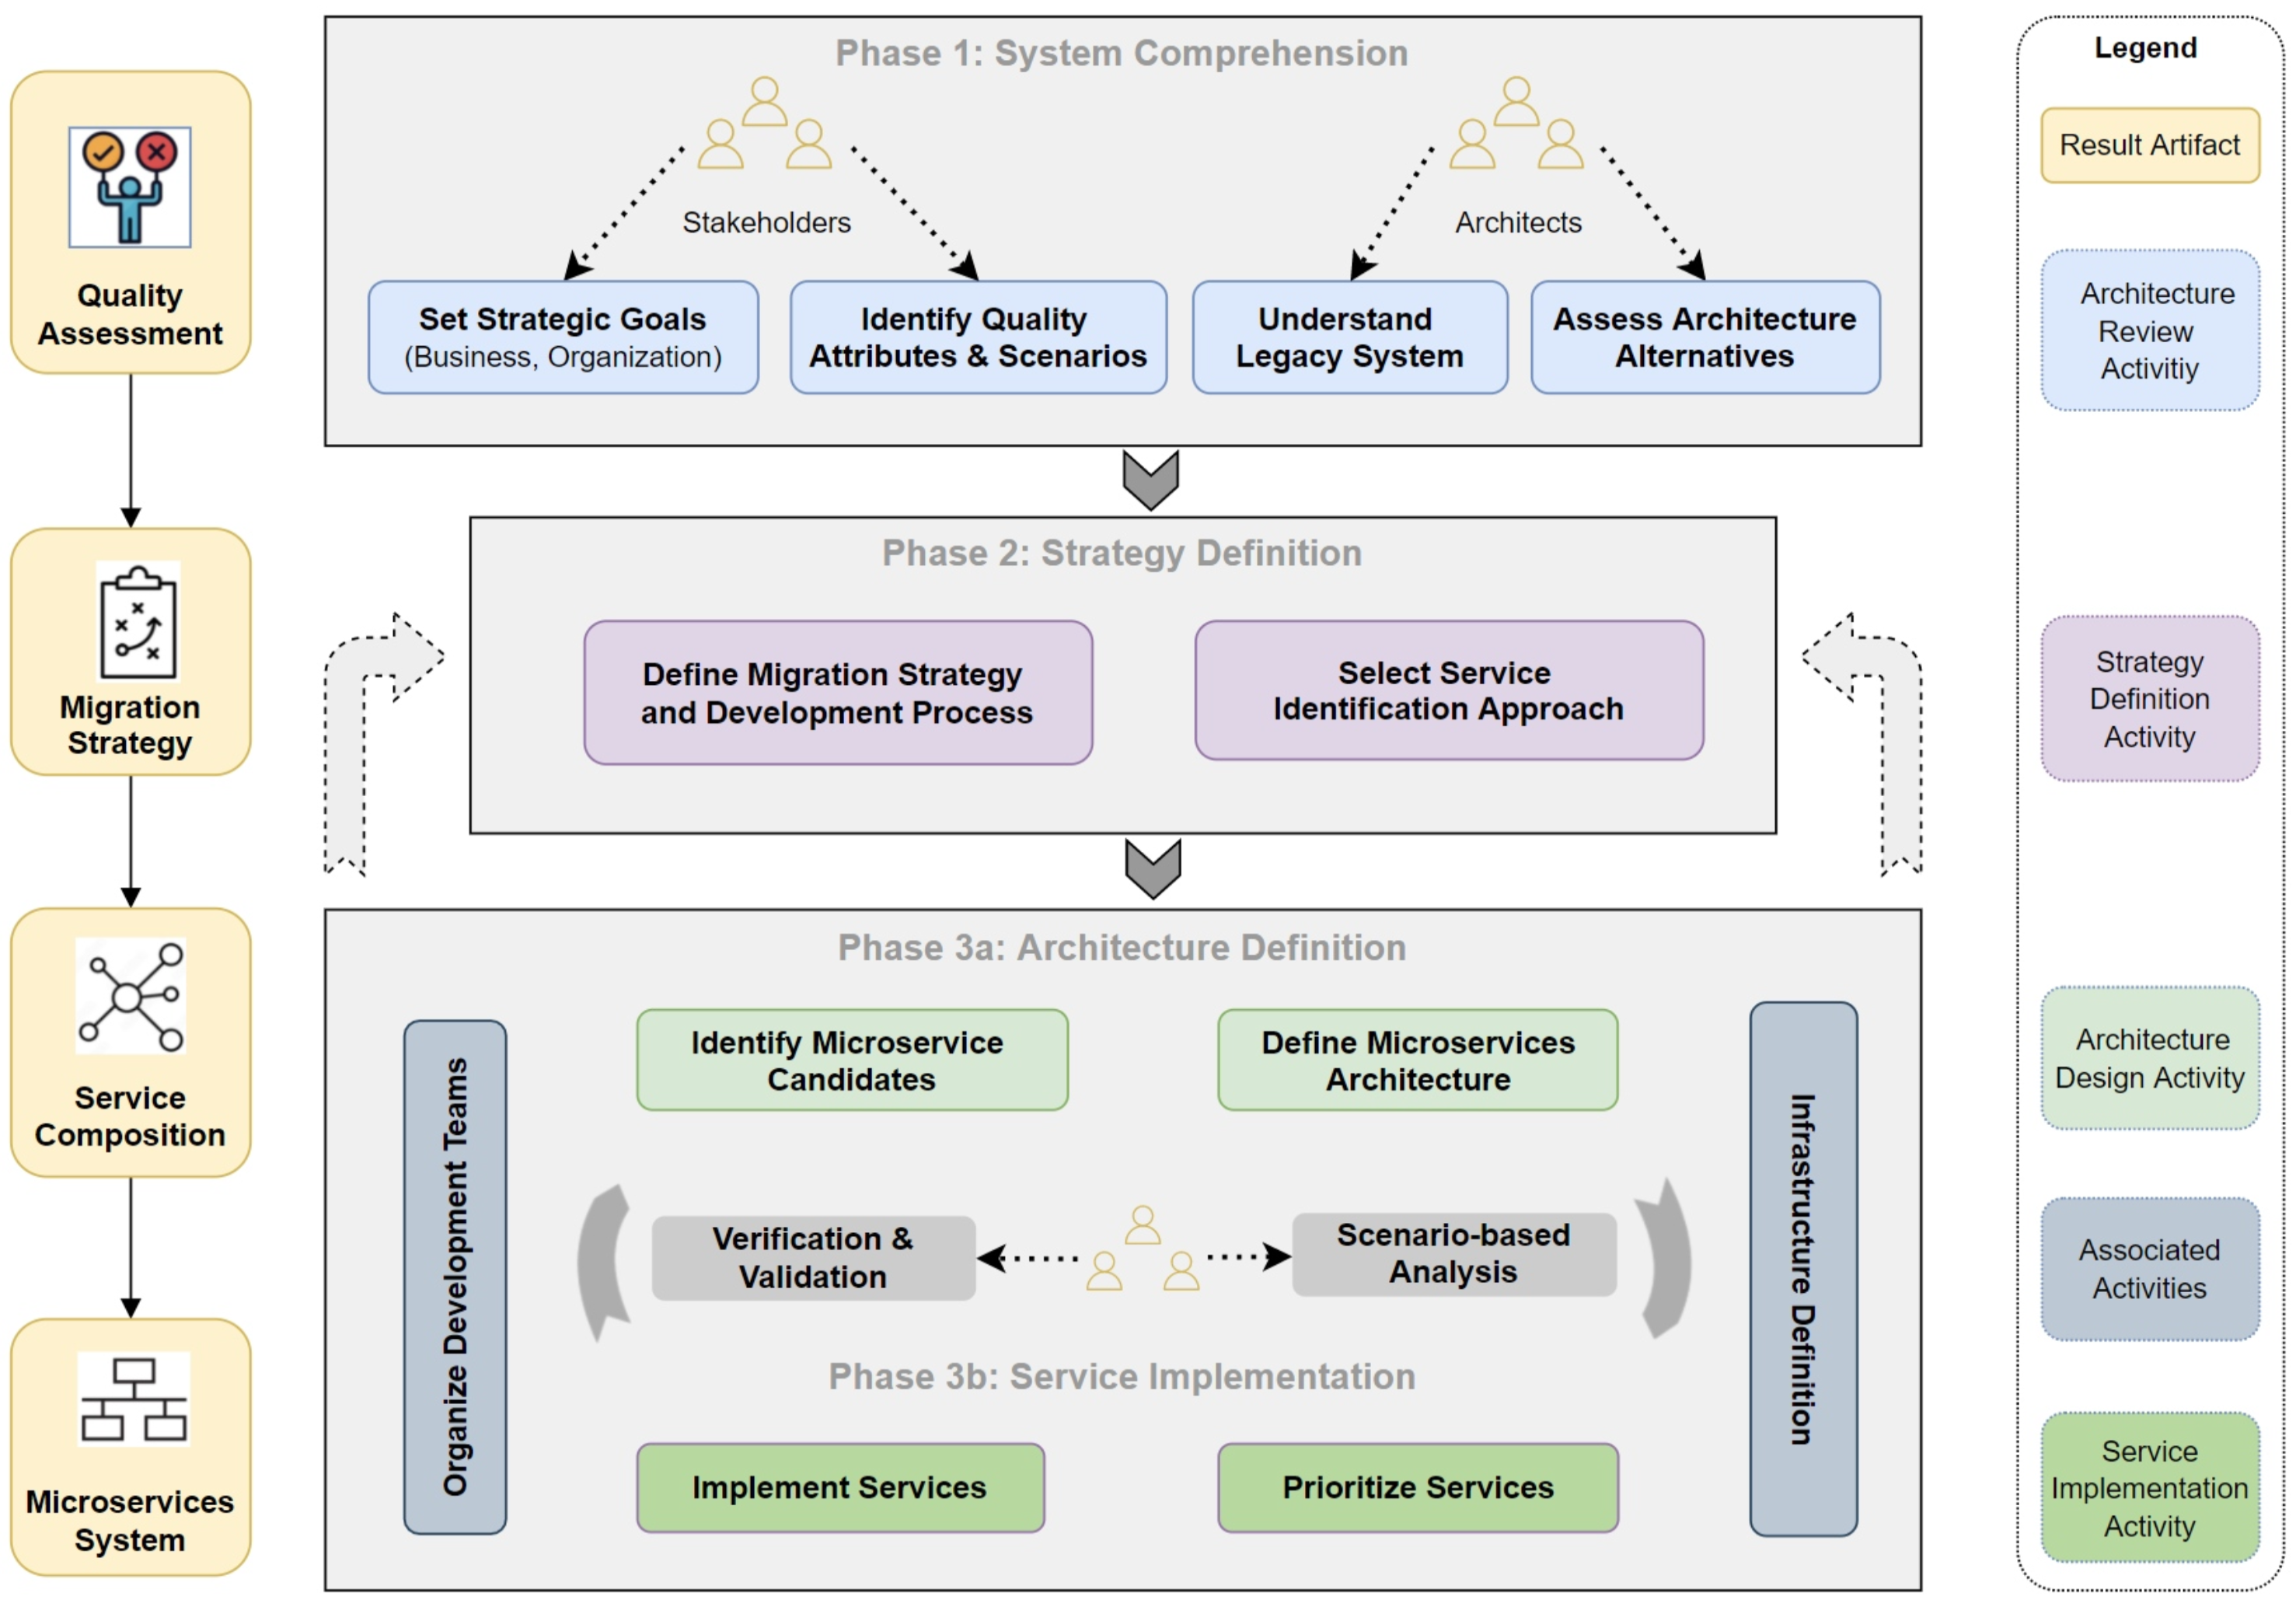
\includegraphics[width=\textwidth]{mmf-overview}
	\caption[\acrfull{mmf} Übersicht]{
		Übersicht über das \gls{mmf} des \gls{ese}
	}
	\label{fig:expert-material-mmf-overview}
\end{figure}

\begin{itemize}
	\item \textbf{Phase 1: System Comprehension:}
	In Phase 1 wird das Verständnis des Systems, das migriert werden soll, angestrebt.
	Mit den Stakeholdern werden dabei strategische Ziele für Produkt und Unternehmen definiert, sowie \glspl{qa} und gewünschte Szenarien identifiziert.
	Es sollen sich dadurch mögliche Treiber für die neue Microservices-Architektur herauskristallisieren.
	Durch das resultierende Verständnis des Systems wird ein Vergleich der alten monolithischen Architektur und einer potentiellen neuen Microservices-Architektur möglich.
	Architekten sollen dann mithilfe dieser Informationen eine Entscheidung für oder gegen die Migration zu Microservices fällen.
	\item \textbf{Phase 2: Strategy Definition:}
	Falls sich in Phase 1 für die Migration zu Microservices entschieden wurde, wird in Phase 2 die Planung der Migration begonnen.
	Die hauptsächliche Aufgabe in dieser Phase ist die Entscheidung, welche Migrationsstrategie benutzt werden soll, um das System zu modernisieren.
	Dafür kann zwischen (momentan) 115 verschiedenen Methoden gewählt werden, die aus akademischen Publikationen stammen.
	Das Werkzeug kann Entwickler dabei unterstützen, indem es basierend auf Eingaben aus Phase 1 empfohlene Methoden vorschlägt.
	Einige dieser Methoden beinhalten die Nutzung von Werkzeugen, welche auch gesondert durchsucht werden können.
	Die verschiedenen Migrationsmethoden und Werkzeuge können von Admins importiert, exportiert und bearbeitet werden, wodurch die Erweiterung in zukünftigen Arbeiten vereinfacht möglich ist.
	\item \textbf{Phase 3a: Architecture Definition:}
	Phase 3 ist in zwei Teile aufgeteilt.
	Im ersten Abschnitt wird die neue Architektur definiert.
	Hier wird, basierend auf der Methode zur Migration, die in der Planungsphase gewählt wurde, der \gls{sia} durchgeführt.
	Außerdem wird allgemeiner die Architektur des gesamten Systems geplant, wobei das Werkzeug Entwickler durch eine Liste von vorgeschlagenen Patterns und Best Practices unterstützen kann.
	Phase 3a und 3b sind eng verbunden, denn durch Erkenntnisse in der Implementierung kann die Planung häufig noch mehrmals überarbeitet werden und dadurch eine neue Implementierung begonnen werden.
	\item \textbf{Phase 3b: Service Implementation:} In Phase 3b startet dann ein Zyklus von Im\-ple\-men\-tie\-rung\-en der in Phase 3a definierten Services.
	Bei Implementierung selbst kann das Werkzeug Entwickler nicht unterstützen.
	Doch Bestandteil der Entwicklungszyklen ist auch, dass das entstehende System anhand der Qualitätsmerkmale zu bewerten.
	Dadurch kann eine unpassende Architekturdefinition oder auch eine unpassende Aufteilung in Services frühzeitig erkannt und korrigiert werden.
	Ist diese Phase abgeschlossen, ist eine erste Version des migrierten Systems fertig.
\end{itemize}

\section{Migrationsverfahren}

In dieser Thesis wurde in Phase 2 des \gls{mmf} eine Suche nach Migrationsverfahren durchgeführt, bei der im Voraus gezielt auf \jf abgestimmte Filter konfiguriert wurden.
Dazu gehören die in Phase 1 des Frameworks erhobenen Szenarien/\glspl{qa} sowie zusätzlich definierte Filter. 
Insgesamt acht dieser Suchergebnisse wurden von mir analysiert und auf ihre Eignung für \jf überprüft.
Davon wurden zwei als potentiell für \jf geeignet bewertet.
In den Interviews sollen Sie ebenfalls eine Einschätzung über die Eignung dieser abgeben.
Deshalb wird deren Funktionsweise im Folgenden beschrieben.

\subsection{Migrationsverfahren 1}

Dieses Verfahren besteht aus drei übergeordneten Schritten (Übersicht in \cref{fig:interviews-migrationsverfahren1}).
\begin{figure}[!ht]
	\centering
	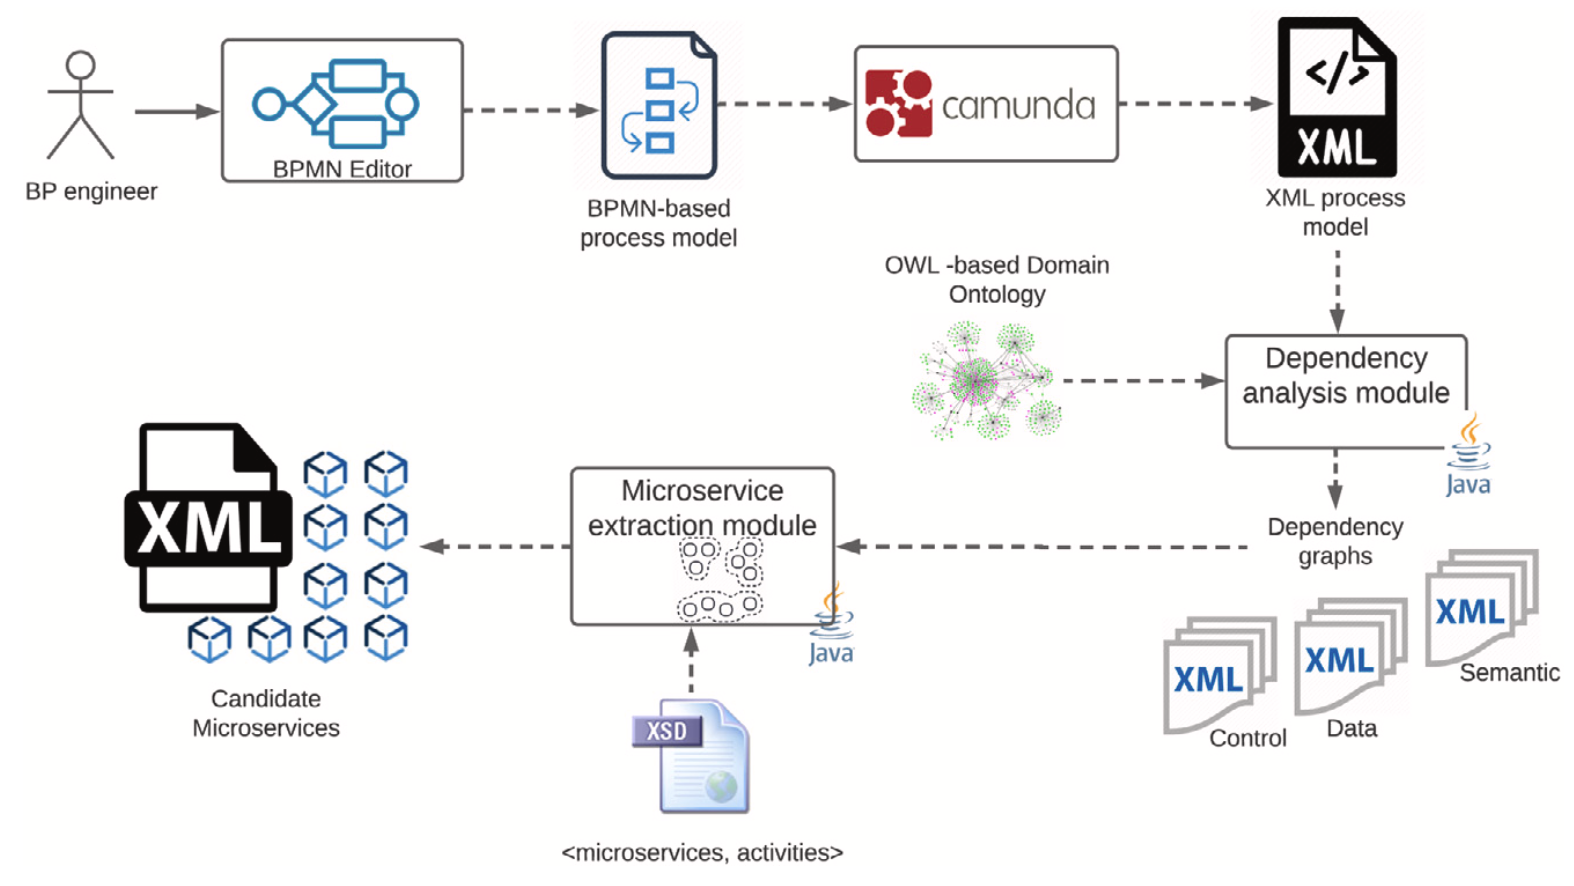
\includegraphics[width=1.0\textwidth]{2_DEF+21_overview}
	\caption[Funktionsweise Migrationsverfahren 1]{
		Funktionsweise des Migrationsverfahren 1. Quelle: \url{https://doi.org/10.1016/j.sysarc.2021.102200}
	}
	\label{fig:interviews-migrationsverfahren1}
\end{figure}
Im ersten Schritt werden die Eingaben für die Methode in Form von \glspl{bp} gesammelt und logisch verbunden, beispielsweise in Form eines \gls{bpmn}-Diagramms (Beispielhafte Eingabe für \jf in \cref{fig:interview-eingabe-verfahren1}).

\begin{figure}[!ht]
	\centering
	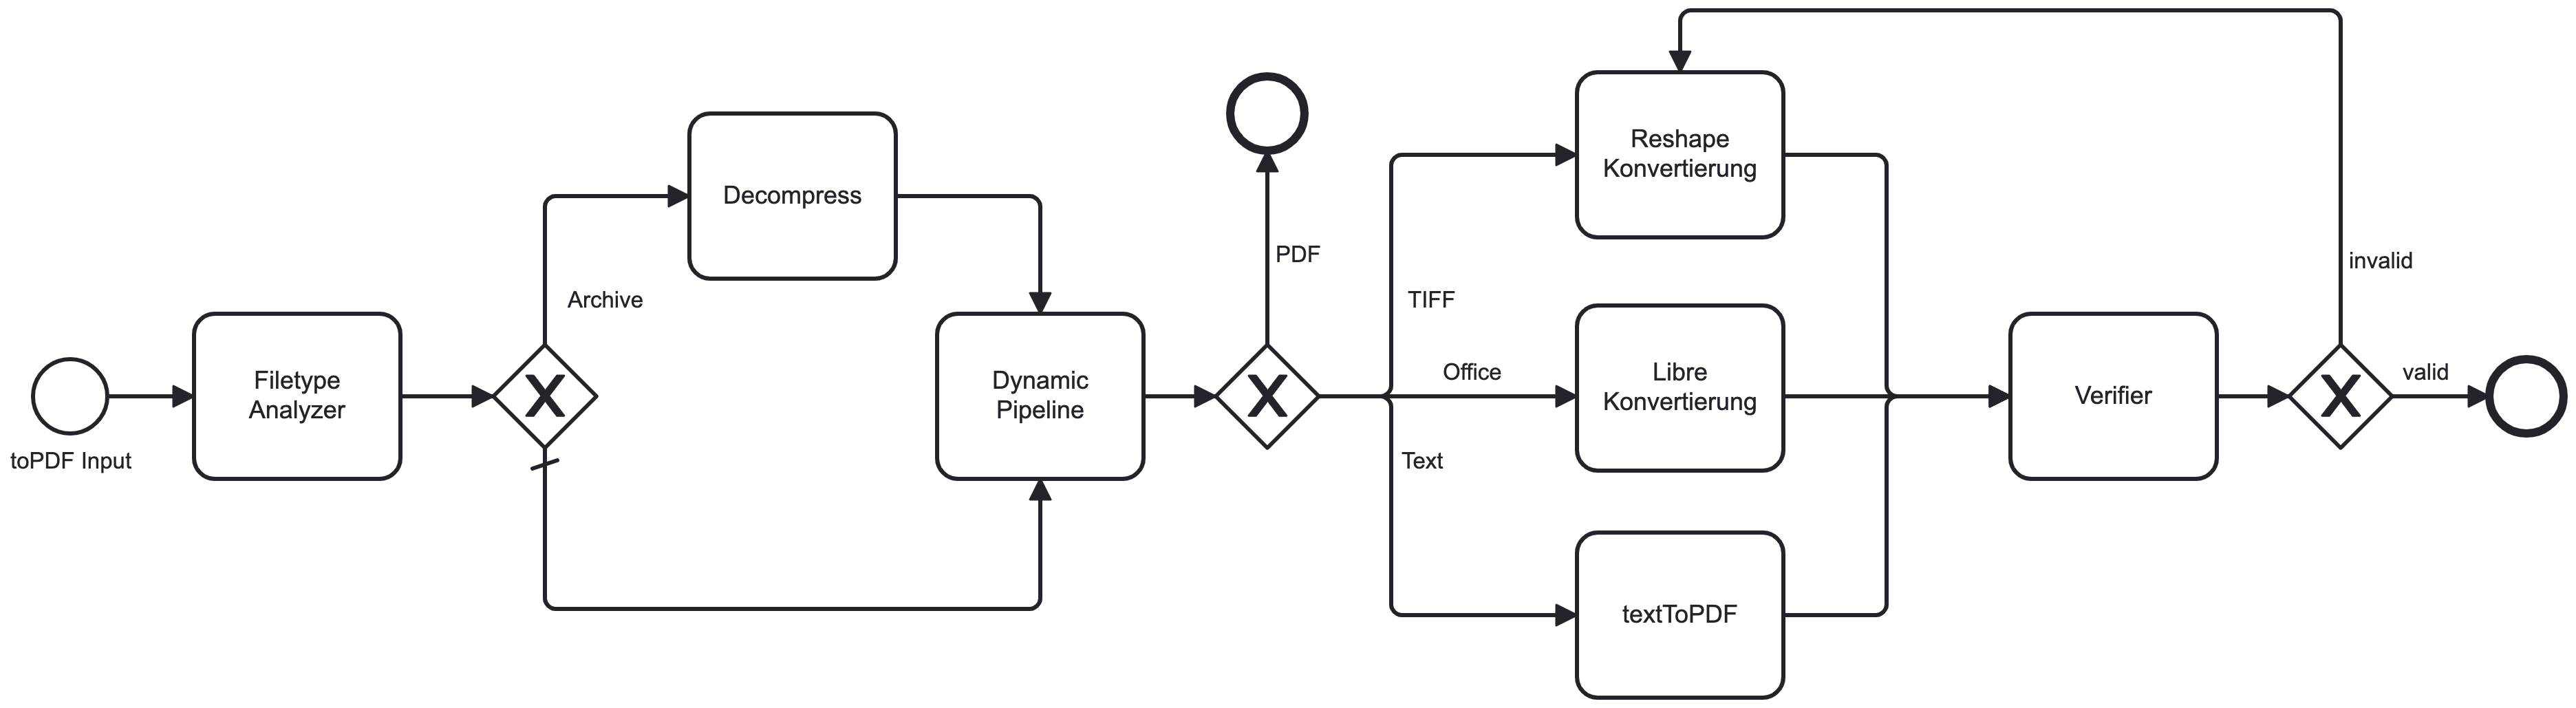
\includegraphics[width=1.0\textwidth]{toPDF_workflow}
	\caption[Mögliche Eingabe Migrationsverfahren 1]{
		Mögliche Eingabe für Migrationsverfahren 1
	}
	\label{fig:interview-eingabe-verfahren1}
\end{figure}

Für die Bestandteile dieser Eingabe (genannt Aktivitäten) werden im zweiten Schritt Abhängigkeiten in drei verschiedenen Formen analysiert: \emph{control dependencies}, \emph{data dependencies} und \emph{semantic dependencies}.
\begin{itemize}
	\item Eine \emph{control dependency} beschreibt eine Abhängigkeit zweier Aktivitäten im Kontrollfluss, also dass eine der Aktivitäten mit hoher Wahrscheinlichkeit auf die andere folgt.
	\item Eine \emph{data dependency} bildet einen Datenfluss zwischen den Ein- oder Ausgaben zweier Aktivitäten ab.
	\item Eine \emph{semantic dependency} gibt die Verwandtschaft des Zwecks zweier Aktivitäten an.
	Die Messung solcher Abhängigkeiten kann anhand der Ähnlichkeit der Namen der Aktivitäten erfolgen.
\end{itemize}

Schließlich wird die \emph{Machine Learning}-Technik \emph{Collaborative Clustering} verwendet, um die Menge von Aktivitäten in Gruppen (genannt \emph{Cluster}) zu unterteilen.
Dabei werden die beschriebenen Metriken verwendet, um die Gruppierung anhand dieser zu optimieren.
Das bedeutet, dass Abhängigkeiten zwischen Aktivitäten des gleichen Clusters gering sein sollten und clusterübergreifend größer sein sollten.

\subsection{Migrationsverfahren 2}

In diesem Verfahren wird das Tool \emph{\acrfull{mb}} vorgestellt, das ein semiautomatisches Modell zur Bewertung der Granularität einer \gls{msa} anbietet (Übersicht in \cref{fig:interviews-migrationsverfahren2}).

\begin{figure}[!ht]
	\centering
	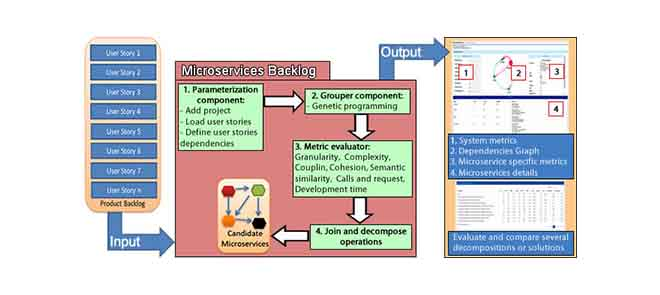
\includegraphics[width=0.7\textwidth]{3_VPAG21-overview}
	\caption[Funktionsweise Migrationsverfahren 2]{
		Funktionsweise des Migrationsverfahren 2. Quelle: \url{https://doi.org/10.1109/ACCESS.2021.3106342}, lizensiert mit \hyperref{https://creativecommons.org/licenses/by/4.0/}{}{}{CCBY} 
	}
	\label{fig:interviews-migrationsverfahren2}
\end{figure}

Als Eingabe werden \emph{User Stories} aus dem \emph{Product Backlog} oder der Release-Planung verwendet.
Diese haben im Vergleich zum ersten Verfahren eine etwas andere Form, aber die Eingaben sind trotzdem mit denen des ersten Verfahrens vergleichbar; mit den User Stories werden auch übliche Workflows beschrieben.
Deswegen wird hier keine Beispielhafte Eingabe vorgestellt.
Außerdem kann \gls{mb} die Metriken  \emph{Coupling}, \emph{Kohäsion}, \emph{Granularität}, \emph{semantische Ähnlichkeit} und \emph{Komplexität} für das Gesamtsystem und für einzelne Microservices berechnen. 
Diese können ebenfalls visualisiert und so übersichtlich betrachtet werden.
Anhand dieser Metriken könnte eine manuelle Überarbeitung der Serviceaufteilung angestoßen werden oder der genetische Algorithmus genutzt werden, der ebenfalls in dem Verfahren vorgestellt wird, um eine Verbesserung der Metriken zu erreichen. 

\chapter{Feldnotizen}
\label{chap:field-notes}

%\fieldnote
%{F1\_P2\_11\_20\_2023\_Activity}
%{test}
%{Datum, Uhrzeit}
%{Ort}
%{Personen}
%{Phase Schritt MMF}
%{
%	aaaaaaa aaaaaa aaaaaa aaaaaaa aaaaaa aaaaaa aaaaaaa aaaaaa aaaaaa aaaaaaa aaaaaa aaaaaa aaaaaaa aaaaaa aaaaaa aaaaaaa aaaaaa aaaaaa aaaaaaa aaaaaa aaaaaa aaaaaaa aaaaaa aaaaaa aaaaaaa aaaaaa aaaaaa aaaaaaa aaaaaa aaaaaa aaaaaaa aaaaaa aaaaaa aaaaaaa aaaaaa aaaaaa aaaaaaa aaaaaa aaaaaa aaaaaaa aaaaaa aaaaaa aaaaaaa aaaaaa aaaaaa aaaaaaa aaaaaa aaaaaa aaaaaaa aaaaaa aaaaaa aaaaaaa aaaaaa aaaaaa aaaaaaa aaaaaa aaaaaa aaaaaaa aaaaaa aaaaaa aaaaaaa aaaaaa aaaaaa aaaaaaa aaaaaa aaaaaa aaaaaaa aaaaaa aaaaaa aaaaaaa aaaaaa aaaaaa aaaaaaa aaaaaa aaaaaa aaaaaaa aaaaaa aaaaaa aaaaaaa aaaaaa aaaaaa aaaaaaa aaaaaa aaaaaa aaaaaaa aaaaaa aaaaaa aaaaaaa aaaaaa aaaaaa aaaaaaa aaaaaa aaaaaa aaaaaaa aaaaaa aaaaaa aaaaaaa aaaaaa aaaaaa aaaaaaa aaaaaa aaaaaa aaaaaaa aaaaaa aaaaaa aaaaaaa aaaaaa aaaaaa aaaaaaa aaaaaa aaaaaa aaaaaaa aaaaaa aaaaaa aaaaaaa aaaaaa aaaaaa aaaaaaa aaaaaa aaaaaa aaaaaaa aaaaaa aaaaaa aaaaaaa aaaaaa aaaaaa aaaaaaa aaaaaa aaaaaa aaaaaaa aaaaaa aaaaaa aaaaaaa aaaaaa aaaaaa aaaaaaa aaaaaa aaaaaa aaaaaaa aaaaaa aaaaaa aaaaaaa aaaaaa aaaaaa aaaaaaa aaaaaa aaaaaa aaaaaaa aaaaaa aaaaaa aaaaaaa aaaaaa aaaaaa aaaaaaa aaaaaa aaaaaa aaaaaaa aaaaaa aaaaaa aaaaaaa aaaaaa aaaaaa aaaaaaa aaaaaa aaaaaa aaaaaaa aaaaaa aaaaaa aaaaaaa aaaaaa aaaaaa aaaaaaa aaaaaa aaaaaa aaaaaaa aaaaaa aaaaaa aaaaaaa aaaaaa aaaaaa aaaaaaa aaaaaa aaaaaa aaaaaaa aaaaaa aaaaaa aaaaaaa aaaaaa aaaaaa aaaaaaa aaaaaa aaaaaa aaaaaaa aaaaaa aaaaaa aaaaaaa aaaaaa aaaaaa aaaaaaa
%}
%{
%	Kommentare
%}
%{
%	Was lief gut
%}
%{
%	Probleme
%}
%{
%	Empfindungen
%}

\fieldnote
{F01\_P2\_11\_20\_2023\_FilterAuswahl}
{1}
{20.11.2023, 10:00-10:30}
{Holzgerlingen, Büro levigo}
{Axel Herrmann, Product Owner}
{2, Einstellen der Filter des \gls{arh}}
{
	Es wurden Filter für die Suche nach Refactoring-Methoden mit dem \gls{arh} eingestellt.
	Dabei wurden die \glspl{sp} als am wichtigsten betrachtet, weswegen dort einige Eigenschaften inkludiert wurden.
	Bei den anderen Kategorien wurde versucht, nur die wichtigsten Filter zu verwenden, da mit zu vielen Filtern eine geringere Aussagekraft dieser vermutet wird.
	Vor allem \emph{Process Preferences} und \emph{Usability Preferences}, also Eigenschaften, die die interne Funktionsweise der Methode betreffen, wurden als relativ unwichtig und vor allem auch unabhängig vom betreffenden System eingestuft und demnach nur ein einziger dieser Filter verwendet.
	Am wichtigsten neben den \glspl{sp} wurden \emph{Input Preferences} und \emph{Output Preferences} eingestuft, da diese ebenfalls stark vom System abhängen und Ausgangslage und gewünschtes Ergebnis betreffen.
	Daraus sind die folgenden Filter resultiert:
	\begin{tabular}{|p{4.5cm}|p{5.5cm}|}
		\hline
		\textbf{Kategorie} & \textbf{Filter} \\ \hline
		Quality Preferences, System Properties & Autonomy, Complexity, Granularity, Isolation, Technology Heterogenity \\ \hline
		Input preferences, Domain Artifacts & Human Expertise, Version Control System \\ \hline
		Input preferences, Execut-ables & API/Interface, Source Code (Java) \\ \hline
		Process preferences, Process Strategy & Refactor \\ \hline
		Output preferences, Repre-sentation & List of services, Splitting recom-mendations \\ \hline
		Usability Preferences & - \\ \hline
	\end{tabular}
}
{
	Die Filter sind noch nicht unbedingt final. Nach einer Durchsicht der Ergebnisse der Refactoring-Methoden kann eine weitere Anpassung der Filter erfolgen.
}
{
	Die Auswahl der Filter mit dem ARH ist simpel, bietet gute UX.
}
{
	Nicht alle Filterkriterien sind direkt verständlich und beinhalten oft noch keine Beschreibung. Beispiel: \emph{Validation Methods} könnte auch so verstanden werden, dass es auf die Validierung des Systems nach Migration bezieht, bezieht sich aber darauf, wie jeweiligen Methoden bereits validiert wurden.
}
{
	Bei manchen Filterkriterien unsicher bezüglich der Bedeutung, legt sich allerdings nach Diskussion darüber.
	Außerdem etwas unsicher, wie genau die Feldnotizen funktionieren werden, da es die erste Anwendung dieser ist.
}

\fieldnote
{F02\_P2\_11\_22\_2023\_FilterAuswahl}
{2}
{22.11.2023, 14:00-14:10}
{Zuhause, Online-Meeting}
{Axel Herrmann, Jonas Fritzsch}
{2, Einstellen der Filter des \gls{arh}}
{
	Die Filter, die in der ersten Feldnotiz angelegt wurden, wurden hier besprochen und im Rahmen dessen der Filter \emph{Source Code (No specification)} hinzugefügt.
  Des Weiteren wurde beschlossen, dass in einem erneuten Treffen mit dem \gls{po} die Filter in zwei Prioritäten unterteilt werden sollen.
}
{}
{Bis auf die eine Änderung wurden die Filter und Entscheidungen dafür für sinnvoll befunden.}
{}
{Zuversichtlich durch die Bestätigung durch den Betreuer.}

\fieldnote
{F03\_P2\_11\_27\_2023\_FilterPrio}
{3}
{27.11.2023, 11:00-11:10}
{Holzgerlingen, Büro levigo}
{Axel Herrmann, Product Owner}
{2, Einstellen der Filter des \gls{arh}}
{
	Die Einstellung der Filter für die Suche nach Refactoring-Methoden mit dem \gls{arh} wurde fortgesetzt.
	Dabei sollten Filter in zwei Prioritäten entstehen, sodass später eine Suche mit allen Filtern und eine mit nur den wichtigsten Filtern durchgeführt werden kann.
	Größtenteils wurden die bereits ausgewählten Filter in die zwei Prioritäten unterteilt, aber in zwei Fällen auch neue, vorher nicht ausgewählte Filter zur geringeren Priorität hinzugefügt.
	Die neuen Filter sind:
	\begin{tabular}{|p{3cm}|p{3.5cm}|p{3cm}|}
		\hline
		\textbf{Kategorie} & \textbf{Filter Prio 1} & \textbf{Filter Prio 2} \\ \hline
		Quality Preferences, System Properties & Autonomy, Granularity, Technology Heterogenity & Complexity, Isolation \\ \hline
		Input Preferences, Domain Artifacts & Human Expertise & Version Control System \\ \hline
		Input Preferences, Runtime Artifacts & & Log Traces \\ \hline
		Input Preferences, Executables & API/Interface, Source Code (No specifica\-tion) & Source Code (Java) \\ \hline
		Process Preferences, Process Strategy & Refactor & \\ \hline
		Output Preferences, Representation & List of services, Split\-ting recommendations & Guideline/ Workflow \\ \hline
		Usability Preferences & - & \\ \hline
	\end{tabular}
}
{
	Die Filter sind vorerst finalisiert. Nach einer Durchsicht der Ergebnisse der Refactoring-Methoden könnten weitere Anpassung der Filter erfolgen.
}
{
	Es konnte sich bei jedem Filter schnell geeinigt werden und die Aufgabe war schnell erledigt.
}
{}
{
	Sicherheit bei der Aufgabe, da das Vorgehen nun klarer ist und alles mit dem Betreuer besprochen wurde.
	Außerdem mehr Sicherheit mit Dokumentation in Feldnotizen.
}

\fieldnote
{F04\_P2\_12\_13\_2023\_Ergebnisbetrachtung}
{4}
{13.12.2023, 13:00-15:00}
{Zuhause}
{Axel Herrmann}
{2, Betrachtung des ersten Suchergebnisses}
{
	Die Arbeit von \Citet{arh-result-no-filter-1} wurde durchgelesen und zusammengefasst.
}
{
	Nach der Betrachtung der anderen Ergebnisse kann die Arbeit erneut und genauer betrachtet werden.
	Eine Bewertung hinsichtlich des Nutzens für \emph{jadice flow} erfolgt später, wenn mit anderen Ergebnissen verglichen werden kann.
}
{
	Der Artikel ist kurz und prägnant.
}
{}
{
	Erster Eindruck: Die Methode wirkt sehr oberflächlich und wenig spezifisch und scheint sich daher weniger zu eignen.
}

\fieldnote
{F05\_P2\_12\_20\_2023\_Ergebnisbetrachtung\_2}
{5}
{20.12.2023, 15:00-17:30}
{Zuhause}
{Axel Herrmann}
{2, Betrachtung des zweiten Suchergebnisses}
{
	Die Arbeit von \Citet{arh-result-no-filter-3} wurde durchgelesen und zusammengefasst.
}
{
	Nach der Betrachtung der anderen Ergebnisse kann die Arbeit erneut und genauer betrachtet werden.
	Eine Bewertung hinsichtlich des Nutzens für \emph{jadice flow} erfolgt später, wenn mit anderen Ergebnissen verglichen werden kann.
}
{
%	Der Artikel beschreibt die Methode zuerst sehr abstrakt, wodurch eine generelle Einschätzung schnell und einfach durchgeführt werden kann aber auch noch eine spätere, genauere Betrachtung möglich ist, indem der detailiertere Part noch betrachtet wird.
%	Außerdem ist er sehr verständlich, da jeder Schritt anhand der durchgeführten Fallstudie erklärt wird, was sehr anschaulich ist.
  Erster Eindruck: Die Methode wirkt sehr viel spezifischer als die erste und scheint relativ gut zu passen.
}
{}
{
  Froh, einen relativ gut passenden Ansatz gefunden zu haben, nachdem der erste nicht gut war.
}

\fieldnote
{F06\_P2\_12\_20\_2023\_Ergebnisbetrachtung\_3}
{6}
{20.12.2023, 17:30-18:30}
{Zuhause}
{Axel Herrmann}
{2, Betrachtung des dritten Suchergebnisses}
{
	Die Arbeit von \Citet{arh-result-no-filter-2} wurde durchgelesen und zusammengefasst.
}
{
	Nach der Betrachtung der anderen Ergebnisse kann die Arbeit erneut und genauer betrachtet werden.
	Eine Bewertung hinsichtlich des Nutzens für \emph{jadice flow} erfolgt später, wenn mit anderen Ergebnissen verglichen werden kann.
}
{
  Bereits das Abstract des Artikels bietet genug Informationen für eine abstrakte Zusammenfassung und ein grundlegendes Verständnis der Methode.
}
{}
{
	Erster Eindruck: Die Methode wirkt sehr viel spezifischer als die erste und scheint relativ gut zu passen.
}

\fieldnote
{F07\_P2\_12\_21\_2023\_Ergebnisbetrachtung\_4}
{7}
{21.12.2023, 08:30-09:30}
{Zuhause, Online-Meeting}
{Axel Herrmann, Product Owner}
{2, Betrachtung der ersten drei Suchergebnisse}
{
	Die Arbeiten von \Citet{arh-result-no-filter-1}, \Citet{arh-result-no-filter-3} und \Citet{arh-result-no-filter-2} wurden dem Product Owner zusammengefasst und gemeinsam die Möglichkeit der Anwendung auf \emph{jadice flow} diskutiert.
  Dabei wurde eine Ordnung der Ergebnisse hinsichtlich ihrer Nützlichkeit für diese Fallstudie vorgenommen, wobei \Citet{arh-result-no-filter-2} mit Platz 1, \Citet{arh-result-no-filter-3} mit Platz 2 und \Citet{arh-result-no-filter-3} mit Platz 3 abschneidet.
}
{
	Die aufgestellte Platzierung ist in Anbetracht dessen, dass erst 3 der 6 Ergebnisse betrachtet wurden, noch nicht vollständig.
}
{
  Alle der Methoden beinhalten eine nützliche Übersichts-Grafik, wodurch das Beschreiben der Methoden gut funktioniert.
  Bei der Platzierung der Methoden kann einfach und unkopliziert Konsens erreicht werden.
}
{}
{
	Der erste Eindruck des Product Owners stimmt mit der des Autors überein.
}

\fieldnote
{F08\_P2\_01\_10\_2024\_Ergebnisbetrachtung\_5}
{8}
{10.01.2024, 10:00-10:30}
{Büro levigo}
{Axel Herrmann}
{2, Betrachtung des vierten Suchergebnisses}
{
  Die Arbeit von \Citet{arh-result-no-filter-4} wurde durchgelesen und zusammengefasst.
}
{
  Die Betrachtung dieser Arbeit ist im Gegensatz zu den anderen Ergebnissen vermutlich final, da die Verwendung dieser Methode schnell ausgeschlossen werden konnte.
}
{
%  Bereits das Abstract des Artikels bietet genug Informationen für eine abstrakte Zusammenfassung und der Ausschluss der Verwendung dieser kann schnell erfolgen.
}
{
  Erster Eindruck: Die Ziele der Methode passen nicht zu unseren und sie ist technisch vermutlich auch nicht anwendbar.
}
{
}

\fieldnote
{F09\_P2\_01\_10\_2024\_Ergebnisbetrachtung\_6}
{9}
{10.01.2024, 11:00-11:30}
{Büro levigo}
{Axel Herrmann}
{2, Betrachtung des fünften Suchergebnisses}
{
  Die Arbeit von \Citet{arh-result-no-filter-5} wurde durchgelesen und zusammengefasst.
}
{
  Nach der Betrachtung der anderen Ergebnisse kann die Arbeit erneut und genauer betrachtet werden.
}
{
  Erster Eindruck: Das Werkzeug kann nicht verwendet werden, die Methode kommt infrage.
}
{
  Erster Eindruck: Verwendung bringt vermutlich erhöhten Aufwand mit sich, da das fehlende Werkzeug manuell nachgeahmt werden muss.
}
{
}

\fieldnote
{F10\_P2\_01\_11\_2024\_Ergebnisbetrachtung\_7}
{10}
{11.01.2024, 11:00-11:30}
{Büro levigo}
{Axel Herrmann}
{2, Betrachtung des sechsten Suchergebnisses}
{
  Die Arbeit von \Citet{arh-result-important-filter-4} wurde durchgelesen und zusammengefasst.
}
{
  Nach der Absprache mit dem \gls{po} kann die Arbeit erneut und genauer betrachtet werden.
}
{
}
{}
{
  Erster Eindruck: Der Kontext von \gls{iiot} passt nicht zu \emph{jadice flow}, ob die Methode trotzdem sinnvoll sein könnte, bleibt offen.
}

\fieldnote
{F11\_P2\_01\_11\_2024\_Ergebnisbetrachtung\_8}
{11}
{11.01.2024, 14:00-14:30}
{Büro levigo}
{Axel Herrmann, Product Owner}
{2, Vergleich der Suchergebnisse}
{
  Die Arbeiten von \Citet{arh-result-no-filter-4}, \Citet{arh-result-no-filter-5} und \Citet{arh-result-important-filter-4} wurden dem Product Owner zusammengefasst und gemeinsam die Möglichkeit der Anwendung auf \emph{jadice flow} diskutiert.
  Dabei wurde eine Ordnung aller Ergebnisse hinsichtlich ihrer Nützlichkeit für diese Fallstudie vorgenommen, wobei immer noch \Citet{arh-result-no-filter-2} mit Platz 1 und \Citet{arh-result-no-filter-3} mit Platz 2 abschneiden.
}
{
}
{
}
{}
{
  Der erste Eindruck des Product Owners stimmt mit der des Autors überein.
}

\fieldnote
{F12\_P2\_01\_17\_2024\_Ergebnisbetrachtung\_9}
{12}
{17.01.2024, 11:00-11:30}
{Zuhause}
{Axel Herrmann}
{2, Betrachtung des siebten Suchergebnisses}
{
  Die Arbeit von \Citet{arh-result-important-filter-7} wurde durchgelesen und zusammengefasst.
}
{
}
{
}
{}
{
  Erster Eindruck: Einsatz wäre vermutlich möglich, Funktionen als atomare Einheiten scheinen allerdings sehr klein-granular und möglicherweise zu aufwendig.
}

\fieldnote
{F13\_P2\_01\_18\_2024\_Ergebnisbetrachtung\_10}
{13}
{18.01.2024, 10:30-11:00}
{Zuhause}
{Axel Herrmann}
{2, Betrachtung des achten Suchergebnisses}
{
  Die Arbeit von \Citet{arh-result-no-qas} wurde durchgelesen und zusammengefasst.
}
{
}
{
}
{}
{
  Erster Eindruck: Einsatz wäre vermutlich möglich, Klassen als atomare Einheiten scheinen allerdings sehr klein-granular und möglicherweise zu aufwendig.
}

\fieldnote
{F14\_P2\_01\_18\_2024\_Ergebnisbetrachtung\_11}
{14}
{18.01.2024, 11:00-11:30}
{Zuhause, Online-Meeting}
{Axel Herrmann, Product Owner}
{2, Vergleich der Suchergebnisse}
{
  Die Arbeiten von \Citet{arh-result-important-filter-7} und \Citet{arh-result-no-qas} wurden dem Product Owner zusammengefasst und gemeinsam die Möglichkeit der Anwendung auf \emph{jadice flow} diskutiert.
  Da nun voraussichtlich alle potentiellen Methoden betrachtet wurden, wurde diskutiert, welche der Verfahren als erstes fokussiert werden sollte.
  Die ersten zwei Plätze belegen dabei \Citet{arh-result-no-filter-2} und \Citet{arh-result-no-filter-3}.
}
{
}
{
  Schnelles Übereinstimmen bei der Bewertung und Sortierung der Verfahren
}
{
  Nur oberfläches Wissen über die Verfahren reicht nicht aus, um final zu entscheiden, welcher Anstatz verwendet wird.
  Einige Verfahren gelten als semi-automatisch, allerdings sind keine der in den Verfahren beschriebenen Tools zu finden, was den zeitlichen Aufwand bei Einsatz der Verfahren schwerer einschätzbar macht.
}
{
  Unsicherheit, welches der Verfahren wirklcih im zeitlichen Rahmen realistisch anwendbar ist
}

\fieldnote
{F15\_P3\_01\_30\_2024\_Methodenanwendung\_1}
{15}
{30.01.2024, 11:00-17:40}
{Zuhause}
{Axel Herrmann}
{3, Anwendung der ersten Migrationsmethode}
{
  Das \result{3} wurde in vorherigen Schritten als favorisierte Methode ausgewählt.
  Der Artikel dazu wurde genauer betrachtet und das beschriebene Tool \acrfull{mb} gesucht.
  Es konnte keine Veröffentlichung des Tools gefunden werden, lediglich ein GitHub Projekt der Autoren, das den richtigen Namen trug.
  Das Projekt scheint veraltet zu sein, es dauerte einige Zeit, es überhaupt zum Laufen zu bringen.
  Auch nach erfolgreichem Start von \gls{mb} in einem Docker Container konnte das Webtool nicht verwendet werden, da abgesehen von der Startseite jede Sub-Seite Fehler auslöste und nicht aufgerufen werden konnte.
  Da der manuelle Aufwand der Umsetzung dieser Methode als zu hoch bewertet wurde, wurde dieses Verfahren letztendlich verworfen.
}
{
  Nach diesem favorisiertem Verfahren besteht noch bei einem weiteren Verfahren Hoffnung, dass es verwendet werden könnte.
  Dieses wird als nächstes betrachtet.
}
{
}
{
  Das beschriebene Tool ist nicht öffentlich verlinkt, das gefundene GitHub Projekt nicht benutzbar und die Methode manuell in dieser Thesis nicht umsetzbar.
}
{
  Frustration über das Fehlschlagen dieses Verfahrens.
}

\fieldnote
{F16\_P3\_02\_07\_2024\_Methodenanwendung\_2}
{16}
{07.02.2024, 10:00-14:00}
{Zuhause}
{Axel Herrmann}
{3, Anwendung der zweiten Migrationsmethode}
{
  Der Algorithmus \emph{cHAC} nach \result{2} wurde im Detail betrachtet und nach Top-Down Methode angefangen umzusetzen.
  Die Implementierung wurde in Java vorgenommen.
  Für gewisse Details des Pseudo-Codes wurden Java-spezifische Konstrukte verwendet statt der im Algorithmus angegebenen.
  Beispielsweise wurde die Synchronisationsvariable @SIC des Algorithmus durch eine CyclicBarrier\footnote{\url{https://docs.oracle.com/javase/8/docs/api/java/util/concurrent/CyclicBarrier.html}} umgesetzt.
}
{
}
{
  Obwohl der Algorithmus relativ komplex ist, wurde er auf einer abstrakten Ebene verstanden und auf dieser auch umgesetzt.
}
{
  Der Algorithmus ist relativ kompliziert und die Beschreibung dazu fällt kurz aus. Viele Teile mussten sehr oft gelesen werden, bevor Verständnis erlangt werden konnte.
}
{
  Unsicher, ob der Algorithmus umgesetzt werden kann.
}

\fieldnote
{F17\_P3\_02\_08\_2024\_Methodenanwendung\_3}
{17}
{08.02.2024, 10:45-17:00}
{Zuhause}
{Axel Herrmann}
{3, Anwendung der zweiten Migrationsmethode}
{
  Der Algorithmus \emph{cHAC} nach \result{2} wurde weiter versucht umzusetzen.
  Die grobe Struktur war duch den vorherigen Tag bereits vorhanden.
  Nun sollten die einzelnen Schritte, Funktionen und Formeln des Artikels umgesetzt werden.
  Dabei konnte kein Erfolg verzeichnet werden; einige Funktionen waren nicht bis ins Detail beschrieben und ließen Freiraum, einige Formeln definierten Eingabevariablen nicht genau und in einer Formel wurde auch ein Schreibfehler vermutet.
  Dadurch dass die Formeln lediglich genannt, nicht aber begründet oder beschrieben wurden, konnten Unklarheiten nicht geklärt und der Algorithmus so nicht umgesetzt werden.
}
{
}
{
}
{
  Kein Erfolg: Arbeit am Algorithmus muss eingestellt werden.
}
{
  Frustration: Obwohl 2 Suchergebnisse vielversprechend klangen, konnte schlussendlich keines davon verwendet werden.
}

\fieldnote
{F18\_P3\_02\_09\_2024\_Besprechung\_Methodenanwendung}
{18}
{09.02.2024, 14.00-14:15}
{Zuhause, Online-Meeting}
{Axel Herrmann, Product Owner}
{3, Besprechung Anwendung Migrationsverfahren}
{
  Die Ergebnisse der erfolgslosen Anwendung der Migrationsmethoden wurden besprochen und gemeinsam beschlossen, die Arbeit des Refactorings deswegen einzustellen.
  Die anderen Suchergebnisse des \gls{arh} wurden bereits in vorherigen Schritten als wesentlich weniger passend bewertet und deswegen und aus Zeitgründen keine weitere Anwendung in Betracht gezogen.
}
{
}
{
}
{
  Kein Erfolg in dieser Phase: Arbeit am Refactoring muss eingestellt werden.
}
{
  Frustration: Obwohl 2 Suchergebnisse vielversprechend klangen, konnte schlussendlich keines davon verwendet werden.
}

